
%%% Local Variables: 
%%% mode: latex
%%% TeX-master: t
%%% End: 

\chapter{环结构特征}
\label{cha:cycle}


\section{环结构特征}
\label{}

本文提出了一种新的局部不变特征,即环结构特征,以应用于图像内容中存在环结构特征的各类图像,比如建筑物图像、树叶图像、视网膜图像、扇贝贝壳图像等。如图\ref{fig:Example}所示,环结构特征由图像中存在的交叉、分叉点及它们之间的连线构成,建筑物中的水泥框架、树叶中的叶脉、视网膜中的血管、扇贝贝壳纹理都可以形成环结构。通过将环结构描述成特征向量,即可应用于识别、配准等各个领域。

\begin{figure}
\centering
  \begin{minipage}[b]{0.48\textwidth} 
      \centering 
      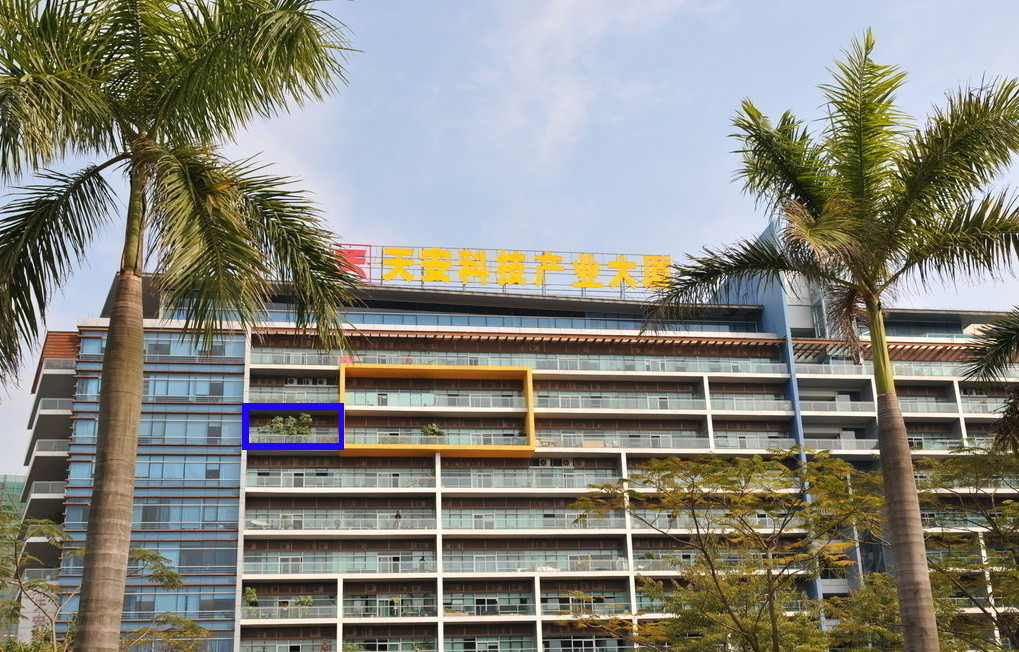
\includegraphics[width=5cm]{building}
        \centerline{(a)}\medskip
    \end{minipage}
  \begin{minipage}[b]{0.48\textwidth}
    \centering
    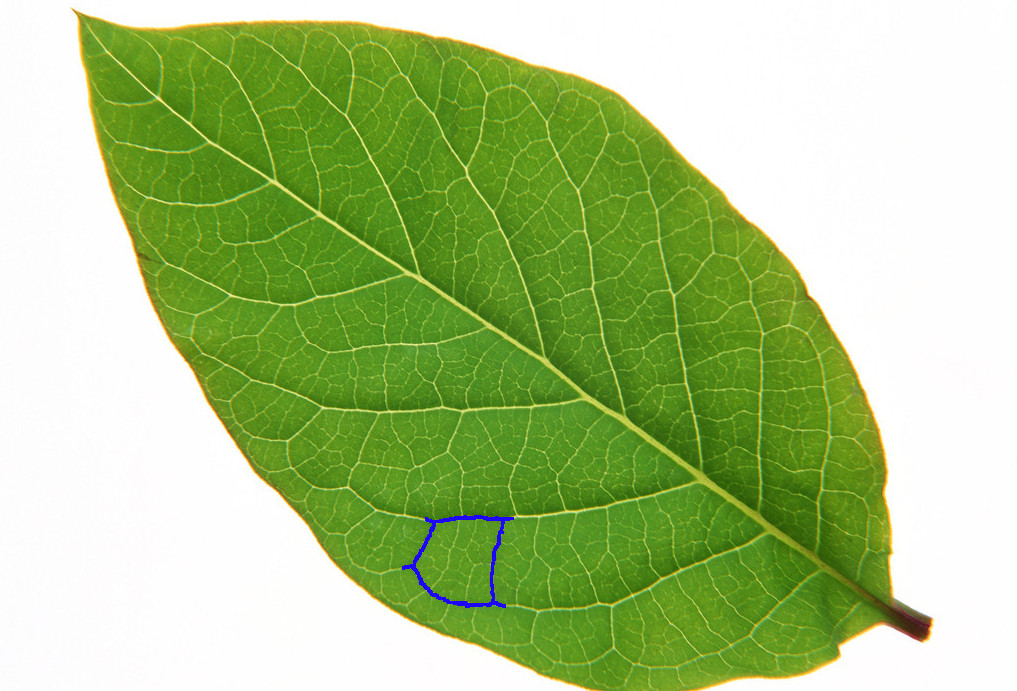
\includegraphics[width=5cm]{reaf}
      \centerline{(b)}\medskip
  \end{minipage}
  \begin{minipage}[b]{0.48\textwidth}
    \centering
    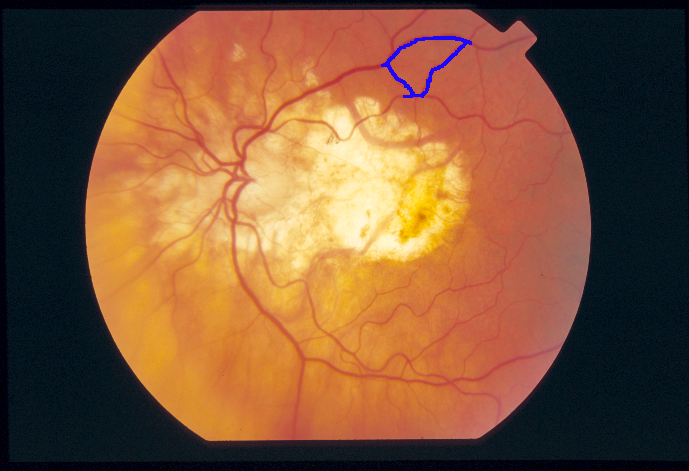
\includegraphics[width=5cm]{retinal}
      \centerline{(c)}\medskip
  \end{minipage}
  \begin{minipage}[b]{0.48\textwidth}
    \centering
    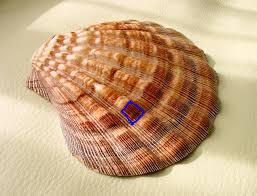
\includegraphics[width=5cm]{scallop}
      \centerline{(d)}\medskip
  \end{minipage}
\caption{图像中的环结构}
\label{fig:Example}
\end{figure}


\section{环与分叉结构检测算法}
\label{}

\subsection{预处理}
\label{}

原始图像一般都是灰度或彩色图像,若想从中提取环结构来用做识别或配准的特征,需要对其进行预处理,以使得环结构特征更加突出,以便能够准确快速的提取。对于原始图像的预处理主要分为四步,即基于偏微分方程的多尺度图像分割、连通区域标记图像去噪、膨胀腐蚀操作填空空洞、骨架化,如图\ref{fig:Preprocessing}所示。经过这四步处理,原始图像中转化为骨架化后的二值图像,以便进行环结构特征的提取。
\begin{figure}
\centering
    \centering
    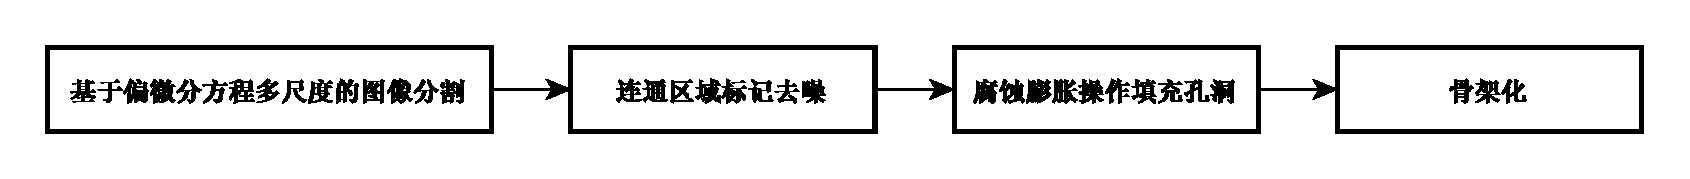
\includegraphics[width=13cm]{preprocessing}\medskip
\caption{预处理流程图}
\label{fig:Preprocessing}
\end{figure}
\subsubsection{基于偏微分方程的多尺度图像分割}

图像分割是计算机视觉领域的至关重要的技术,是介于图像分析与低层图像处理之间的图像处理过程,因而图像分割的结果好坏将很大程度上影响后续对图像的处理及应用。近些年来,对图像分割技术的研究层出不穷,分为基于区域的分割,基于边缘的分割,基于特定理论的分割,如基于模糊理论的分割、基于水平集的分割、基于活动轮廓的分割、基于图论的分割\cite{xuxiaoli}等等。

环结构特征存在于很多类图像中,不同类图像的环结构之间有很大的不同。例如,视网膜血管图像中血管较细、直径宽度变化范围大,血管与背景对比度低,扇贝贝壳纹理图像中边缘较模糊等,这就增加了图像分割的难度。为了减小图像分割对图像配准或识别的影响,并且使分割结果能够适用于多类不同图像,我们采用了基于偏微分方程多尺度的图像分割。

基于偏微分方程的多尺度图像分割\cite{wang2013retinal}不需要预处理与训练,可直接用于各类图像的分割。首先,利用不同多小波核对图像中的边缘进行增强,利用多小波核对不同边缘的反映特性的不同,进行区分处理。通过多尺度多层分解方法对归一化的图像进行处理,以达到去除噪声和定位边缘的目的。尺度不同表示边缘的细化程度不同。最后,采用自适应阈值方法得到分割后的二值图像。这样一幅图像就得到了不同尺度的多个分割结果,针对不同的应用问题就可以选择不同的尺度进行后续处理。

图\ref{fig:Segmentaion-retinal}显示了视网膜图像的三个不同尺度的分割结果,从图中可以看出,尺度越大,越来越多的血管被分割出来。但分割的越精细,噪声也越大。为了消除噪声对环结构提取的影响,我们要对分割后的图像进行去噪处理

\begin{figure}
\centering
  \begin{minipage}[b]{0.48\textwidth} 
      \centering 
      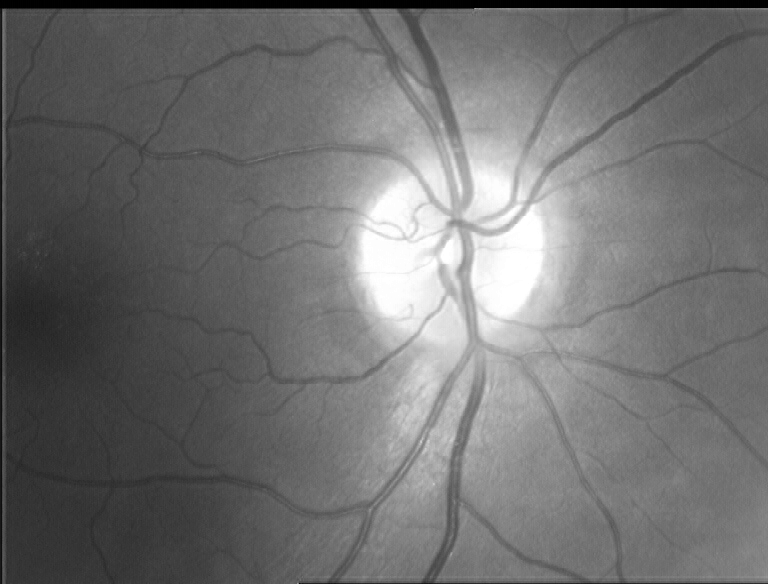
\includegraphics[width=6cm]{118}
        \centerline{(a)}\medskip
    \end{minipage}
  \begin{minipage}[b]{0.48\textwidth}
    \centering
    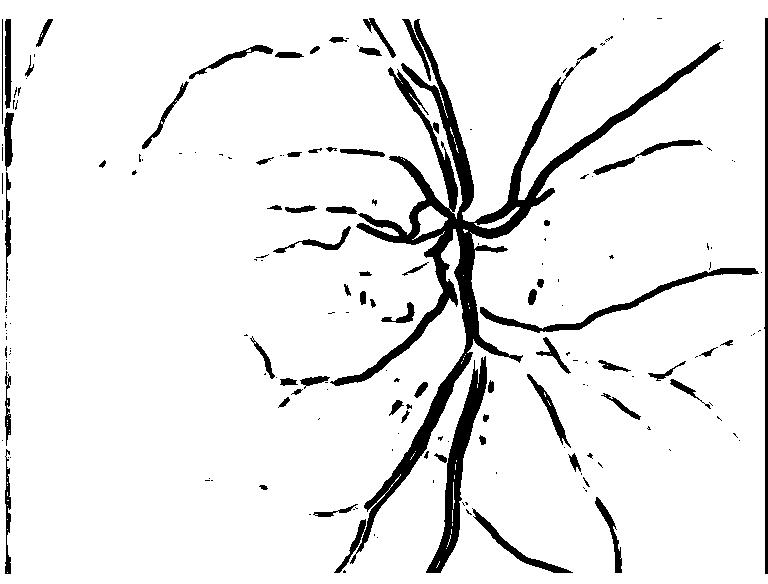
\includegraphics[width=6cm]{118-13}
      \centerline{(b)}\medskip
  \end{minipage}
  \begin{minipage}[b]{0.48\textwidth}
    \centering
    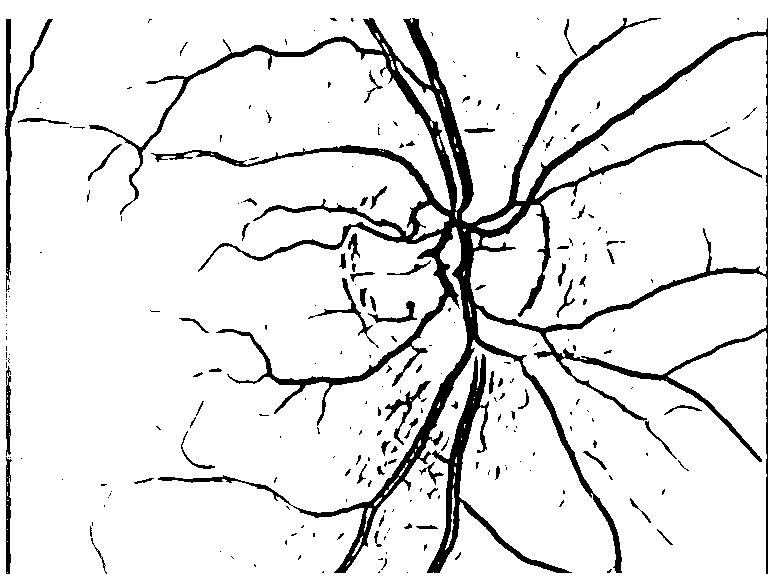
\includegraphics[width=6cm]{118-08}
      \centerline{(c)}\medskip
  \end{minipage}
  \begin{minipage}[b]{0.48\textwidth}
    \centering
    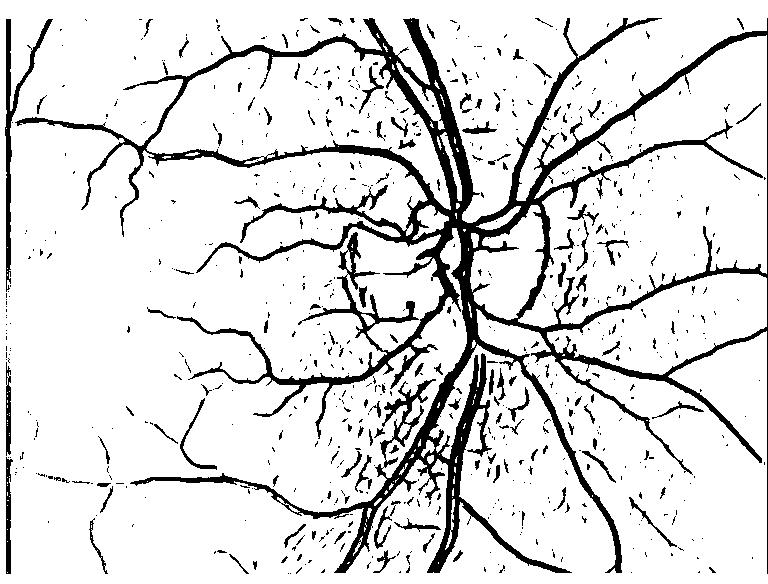
\includegraphics[width=6cm]{118-01}
      \centerline{(d)}\medskip
	\label{fig:max}
  \end{minipage}
\caption{不同尺度的视网膜分割结果}
\label{fig:Segmentaion-retinal}
\end{figure}
\subsubsection{连通区域标记图像去噪}

连通区域标记\cite{xuzhengguang}是图像处理中常用的一个基本方法,在目标分割、边缘检测中有着十分广泛的应用。同时,连通区域也可应用于图像去噪。
采用连通区域算法对连通区域进行标记,即通过对二值图像进行逐行逐列扫描,根据图像中像素之间的邻域关系,对属于同一四连通或八连通区域的像素赋予相同的标号,然后统计同一标号的像素的个数。若像素数小于某个阈值,则认为是噪声。

邻域关系有两种,即四邻域与八邻域。设像素$P(x, y)$,则像素P的四邻域表示为$P_1(x,y-1), P_2(x, y+1), P_3(x-1,y), P_4(x+1,y)$,像素P的八邻域表示为$P_1(x,y-1), P_2(x, y+1), P_3(x-1,y), P_4(x+1,y), P_5(x-1,y-1), P_6(x+1, y+1), P_7(x-1,y+1), P_8(x+1, y-1)$,更加直观的表示如表\ref{tab:adjacent}。为了更好的去除噪声,我们采用八邻域去噪。
\begin{table}
\centering
\caption{四邻域与八邻域}
\begin{tabular}{|c|c|c|}
\hline
 & $P_1$ & \\
\hline            
$P_3$ & $P$ & $P_4$\\
\hline           
& $P_2$ & \\
\hline
\end{tabular}
\begin{tabular}{|c|c|c|}
\hline
$P_5$ & $P_1$ & $P_7$\\
\hline            
$P_3$ & $P$ & $P_4$\\
\hline            
$P_8$& $P_2$ & $P_6$ \\
\hline
\end{tabular}

\label{tab:adjacent}
\end{table}


图\ref{fig:denoise-table}是一幅二值图像的连通区域标记图,从图中可以看出,共有2个连通区域,标号为1、2。其中连通区域1只有两个像素,连通区域2有11个像素,若设定10个像素为基准,小于10个像素的连通区域为噪声,则连通区域1将被认为是噪声,进行去除。\ref{fig:Preprocessing}(b)是图\ref{fig:Segmentaion-retinal}(d)经过去噪后的结果,从图中可以看出很多的噪声都被滤除了。


\begin{figure}[H] % use float package if you want it here
  \centering
  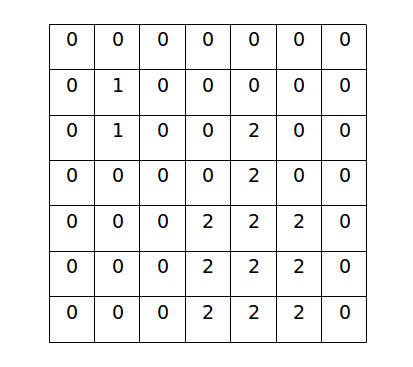
\includegraphics[width=0.4\textwidth]{denoise-table}
  \caption{连通区域去噪}
  \label{fig:denoise-table}
\end{figure}



\subsubsection{膨胀腐蚀操作填空空洞}
在有些情况下,有时图像的亮度值不均匀,这就造成了分割出的线是断裂的或有孔洞的情况,为了骨架化后的图像能准确的体现原图像的特征,需对分割后的图像进行先膨胀后腐蚀操作。
膨胀腐蚀是图像形态学中比较常见的处理,一般是对二值图像进行处理。
用b对函数f进行的灰度膨胀\cite{gang}表示为:
\begin{align}
(f\oplus b)(s,t)=max\{f(s-x, t-y)+b(x,y)|(s-x),(t-y)\in D_f;(x,y)\in D_b\}
\end{align}
其中,$D_f$和$D_b$分别是f和b的定义域。
灰度腐蚀表示为$f \ominus b$,定义为:
\begin{align}
(f \ominus b)(s,t)=min\{f(s+x, t+y)-b(x,y)|(s+x),(t+y)\in D_f;(x,y)\in D_b\}
\end{align}

经膨胀腐蚀操作后,孔洞会被消除,如图\ref{fig:Preprocessing}(c)所示。

\subsubsection{骨架化}
为了获得一个像素宽的骨架化结果,我们采用轮廓修剪骨架提取方法~\footnote{http://www.cs.smith.edu/$\sim$nhowe/research/code/}。这个方法是Nicholas R. Howe实现的,想法是Alex Telea提出的。若一个点位于一个圆圈的中心,并接触一个图像边缘的多个点。灰度骨架化图像的强度是基于围绕图像的周长连接最远的两点的最短距离。因此,骨架中的毛刺是由微小的边缘扰动引起的强度变化。如果圆圈接触断裂的边缘,骨架化将会是无限的过程。最终的骨架化结果是通过噪声突起轮廓的预期大小来确定的阈值来决定的。图\ref{fig:Preprocessing}(d)是骨架化结果,从图中可以看到,骨架后的图像能准确的描绘出血管的主轮廓。
\begin{figure}
\centering
  \begin{minipage}[b]{0.48\textwidth}
    \centering
    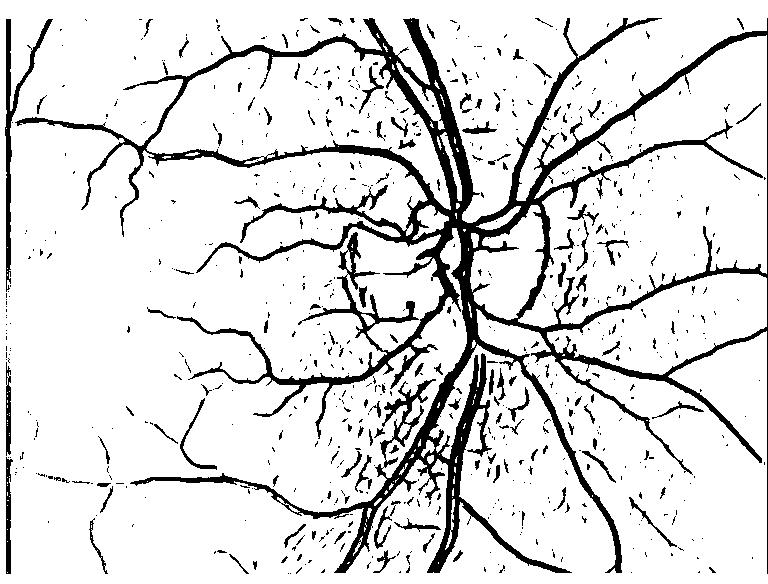
\includegraphics[width=6cm]{118-01}
      \centerline{(a) 分割图}\medskip
  \end{minipage}
  \begin{minipage}[b]{0.48\textwidth}
    \centering
    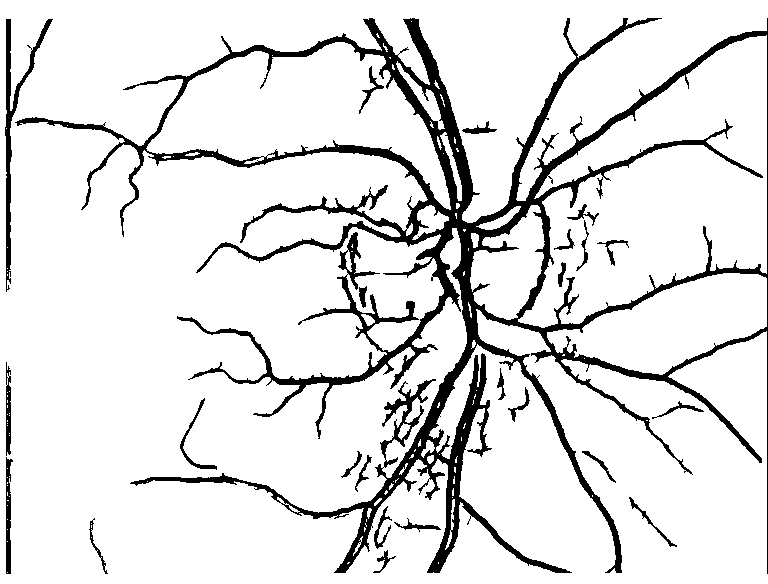
\includegraphics[width=6cm]{denoise}
      \centerline{(b) 去噪图}\medskip
  \end{minipage}
  \begin{minipage}[b]{0.48\textwidth}
    \centering
    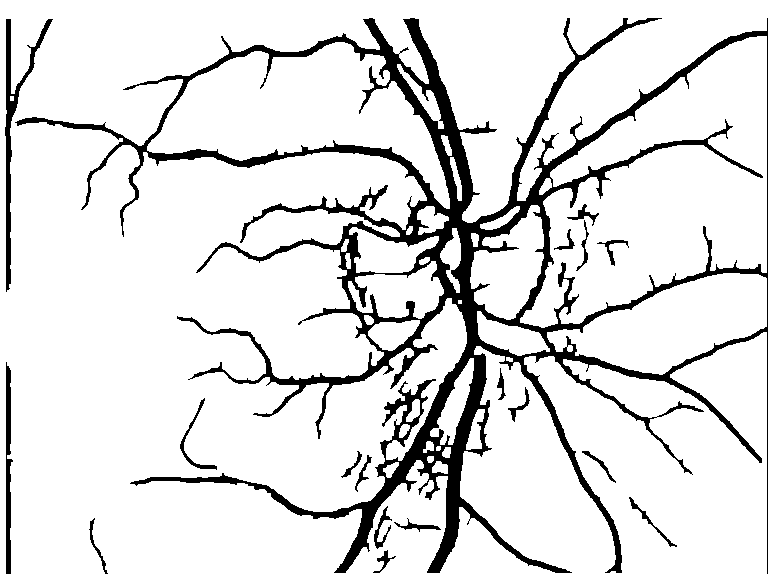
\includegraphics[width=6cm]{fill}
      \centerline{(c) 填充图}\medskip
  \end{minipage}
  \begin{minipage}[b]{0.48\textwidth}
    \centering
    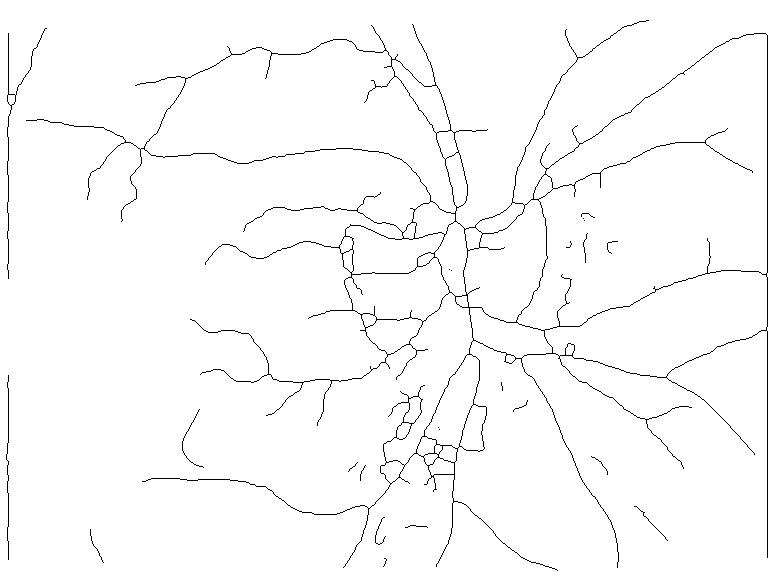
\includegraphics[width=6cm]{118-skel}
      \centerline{(d) 骨架图}\medskip
  \end{minipage}
\caption{预处理}
\label{fig:Preprocessing}
\end{figure}

经过这四个步骤,各类彩色图像就变为去噪后的骨架化二值图像,其中的环结构具有一个像素宽度,这样就为检测环结构做好了准备。

\subsection{算法描述}
\label{}
\subsubsection{图论相关概念}
\label{}

图像中环的概念是由图论扩展而来的。在人类社会的实际生活中,有时在描述某些事物或对象之间有某种特定关系时采用图形的方式显得更加直观。对象用图形中的点表示,两对象之间具有的某种特定的关系用两点之间的无向或有向连线表示,由此数学抽象产成了图的概念。

\begin{definition}
一个图$G$定义为一个数学结构$(V, E, \phi)$\cite{xujunming},其中
\begin{enumerate}
\item $V$是一个集合,其中的元素成为顶点;
\item $E$是定义在$V$上的可以重复的二元关系集,其中的元素成为边;
\item $\phi$ 是$E$到$V$的一个映射。 
\end{enumerate}
若$\phi(E)$中的元素全是有序对,则$(V, E, \phi)$成为有向图,否则,成为无向图。我们所研究的图像中的线是无方向的,所以我们可以把图像认为是无向图。
\end{definition}

在图像中,顶点可以定义为线的交叉、分叉点或孤立点,边为连接两个顶点的连线,如图\ref{fig:graph}所示,$V = \{v_1, v_2, v_3, v_4, v_5\}$,$E = \{e_1, e_2, e_3, e_4\}$,边$e_1$把顶点$v_1, v_2$连接起来。

\begin{figure}[H] % use float package if you want it here
  \centering
  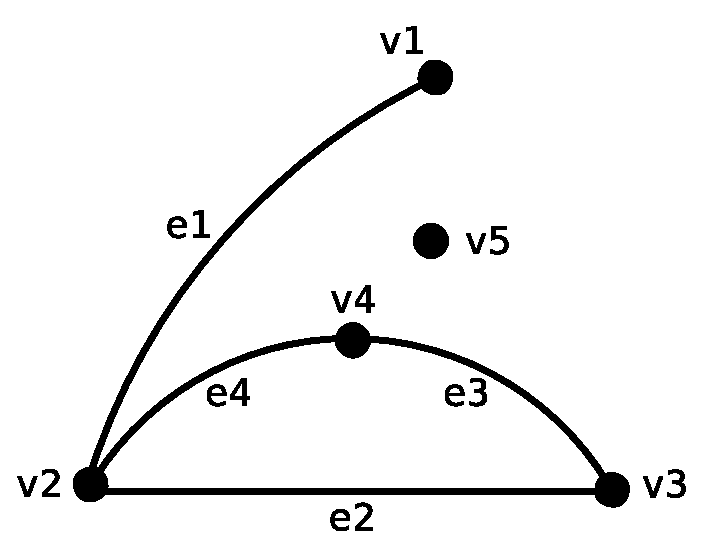
\includegraphics[width=0.3\textwidth]{graph}
  \caption{图}
  \label{fig:graph}
\end{figure}

\begin{definition}
设$G$是无向图,$x\in V(G)$的顶点度定义为$G$中与$x$关联边的数目,记为$d_{G}(x)$\cite{wangshuhe}。
\end{definition}

图\ref{fig:graph}中,只有一条边$e_1$与顶点$v_1$相连,即$d_{v_1}=1$,类似的,$d_{v_2}=3, d_{v_5}=0$。


\begin{definition}
设无向图$G = (V, E), v_i, v_j \in V$,若存在一条边$e$以$v_i, v_j$为端点,即$e = (v_i, v_j)$,则称$v_i, v_j$是彼此相邻的,简称相邻的。 
\end{definition}
例如,图\ref{fig:graph}中,$v_1$与$v_2$是相邻的,$v_2$与$v_5$是不相邻的。

设$(V, E, \phi)$是无向图$G$,其中$V = \{v_1, v_2, \ldots, v_p\}$,$E = \{e_1, e_2, \ldots, e_\varepsilon\}$。则无向图G的邻接矩阵能够反映出V中元素与E中元素之间的关联关系。
\begin{definition}
设图G的顶点集$V = \{v_1, v_2, \ldots, v_p\}$,令
\begin{align}
a_{ij} = \left\{ \begin{array}{ll}
1 & \textrm{$v_i$与$v_j$相邻}\\
0 & \textrm{$v_i$与$v_j$不相邻或$i = j$}
\end{array} \right.
\end{align}
则称由元素$a_{ij} (i, j == 1, 2, \ldots, p)$构成的p阶矩阵为图G的邻接矩阵\cite{wangzhaorui},记作A。
\end{definition}
图\ref{fig:graph}的邻接矩阵是
\begin{align}
A = \left( \begin{array}{lllll}
0 & 1 & 0 & 0 & 0 \\
1 & 0 & 1 & 1 & 0 \\
0 & 1 & 0 & 1 & 0 \\
0 & 1 & 1 & 0 & 0 \\
0 & 0 & 0 & 0 & 0 
\end{array} \right)
\end{align}

无向图中的环是指一系列边的集合,起始点与终止点是重合的。一些环的集合成为一个环基。在无向无权图中,环的权重为组成这个环的边的数量。最小环基就表示能使组成这个环基的权重的总和最小的环的集合。图\ref{fig:graph}中,共存在九个环,即:$c_1 = < v_1, v_2, v_3>, c_2 = <v_4, v_5, v_6>, c_3 = <v_5, v_6, v_7, v_8, v_10>, c_4 = <v_8, v_9, v_10>, c_5 = < c_14, c_15, c_16>, c_6 = <v_10, v_11, v_12, v_13>, c_7 = <c_4, c_5, v_10, v_10, v_8, v_7, v_6>, c_8 = < v_6, v_5, v_10, v_9, v_8, v_7>, v_9 = < v_4, v_5, v_10, v_9, v_8, v_7, v_6>$,其中,$c_1, c_2, c_3, c_4, c_5$是最小环,他们组成的集合为最小环基,即$M = \{c_1, c_2, c_3, c_4, c_5\}$。
\begin{figure}
\centering
    \centering
    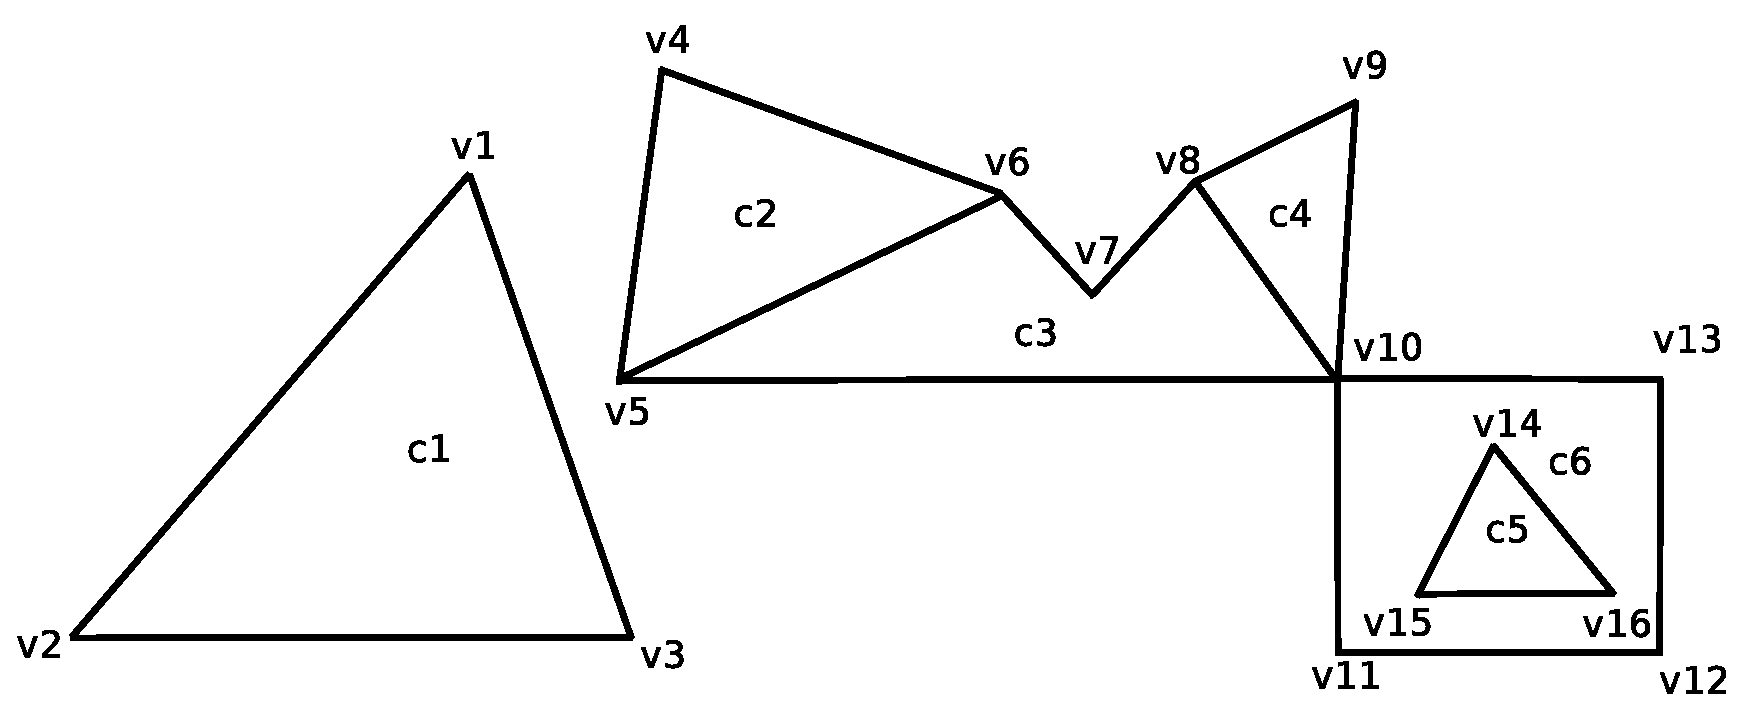
\includegraphics[width=10cm]{graph-cycle}\medskip
\caption{图中的环}
\label{fig:graph-cycle}
\end{figure}


检测图中的所有的环的问题,实际上就是检测图中的最小环基的问题。图\ref{fig:graph}中,$e_2, e_3, e_4$组成一个无向环。
要在图像中检测最小环基,首先应先检测分叉点及其之间的连接关系,根据其连接关系,构造搜索路径,以此来实现检测环的过程。

\subsubsection{检测分叉点与连接关系}
\label{}

二值图像中,若背景为黑,即其像素值是0,线为白,即像素值是1。要判断一个像素点是否为分叉点,首先应定位线的位置,即判断像素值是否为1,然后判断这个像素点的八邻域像素为1的像素个数,若八邻域没有像素为1的像素,则认为是度为1的顶点,即孤立点,若八邻域有1个像素值为1的像素,则认为这两个点形成一条短线段,这些点都不认为是分叉点。这样研究对象为八邻域内有大于等于3个像素值为1的点。通过观察与实验发现若八邻域有3个像素值为1的像素,则中心点其八邻域像素值为1的点形成三分叉,中心点可被认为是三分叉点,如图\ref{fig:FeaturePoints}所示,图(a)中的红色点八邻域内有3个值为1的点,则红色点为三分叉点。三分叉点的常见情况如图\ref{fig:FeaturePoints-image}(a)所示。

而若某一点的八邻域有三个以上像素值为1的像素,则不能单纯的认为是几分叉点,如图\ref{fig:FeaturePoints}(b)所示是四分叉点的例子,红色点及蓝色点八邻域都有3个以上的值为1的点,但蓝色点不能认为是分叉点。

这种情况下,我们要进行连通区域标记。首先重新定位可能是分叉点的点,即其八邻域有3个以上像素值为1的点。然后要进行连通区域标记,图\ref{fig:FeaturePoints}(b)中的红色及蓝色点标记为一个区域,根据标记点的坐标,计算连通区域的中心位置,最后把中心位置点作为同一个连通区域的分叉点,而连通区域内的其他点为普通点,即红色点作为连通区域的中心,看作是真正的四分叉点。在图像中\ref{fig:FeaturePoints}(b)显示为\ref{fig:FeaturePoints-image}(b),通过计算,蓝色点为中心位置点,即四分叉点。

\begin{figure}
\centering
  \begin{minipage}[b]{0.48\textwidth} 
      \centering 
      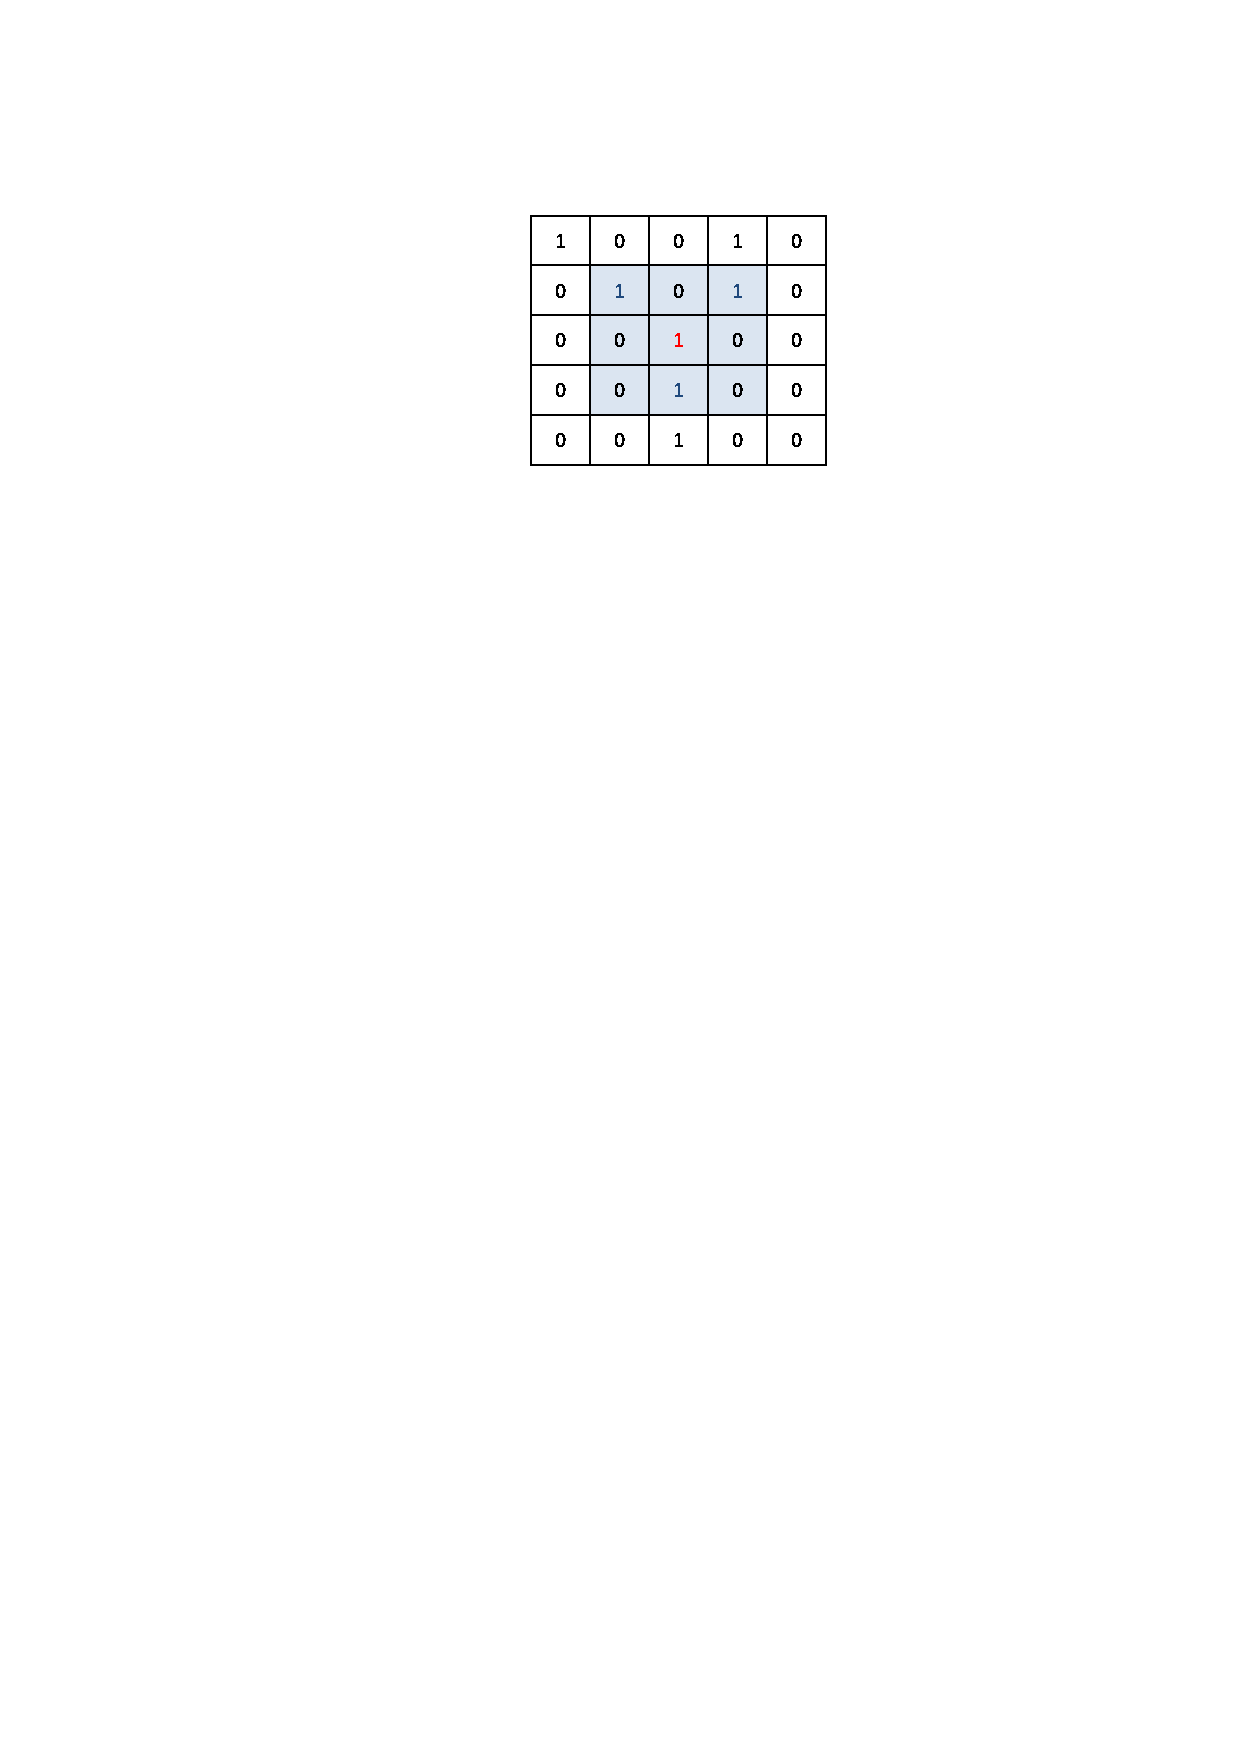
\includegraphics[width=4cm]{3FeaturePoint}
        \centerline{(a)}\medskip
	 \label{fig:3FeaturePoint}
    \end{minipage}
  \begin{minipage}[b]{0.48\textwidth}
    \centering
    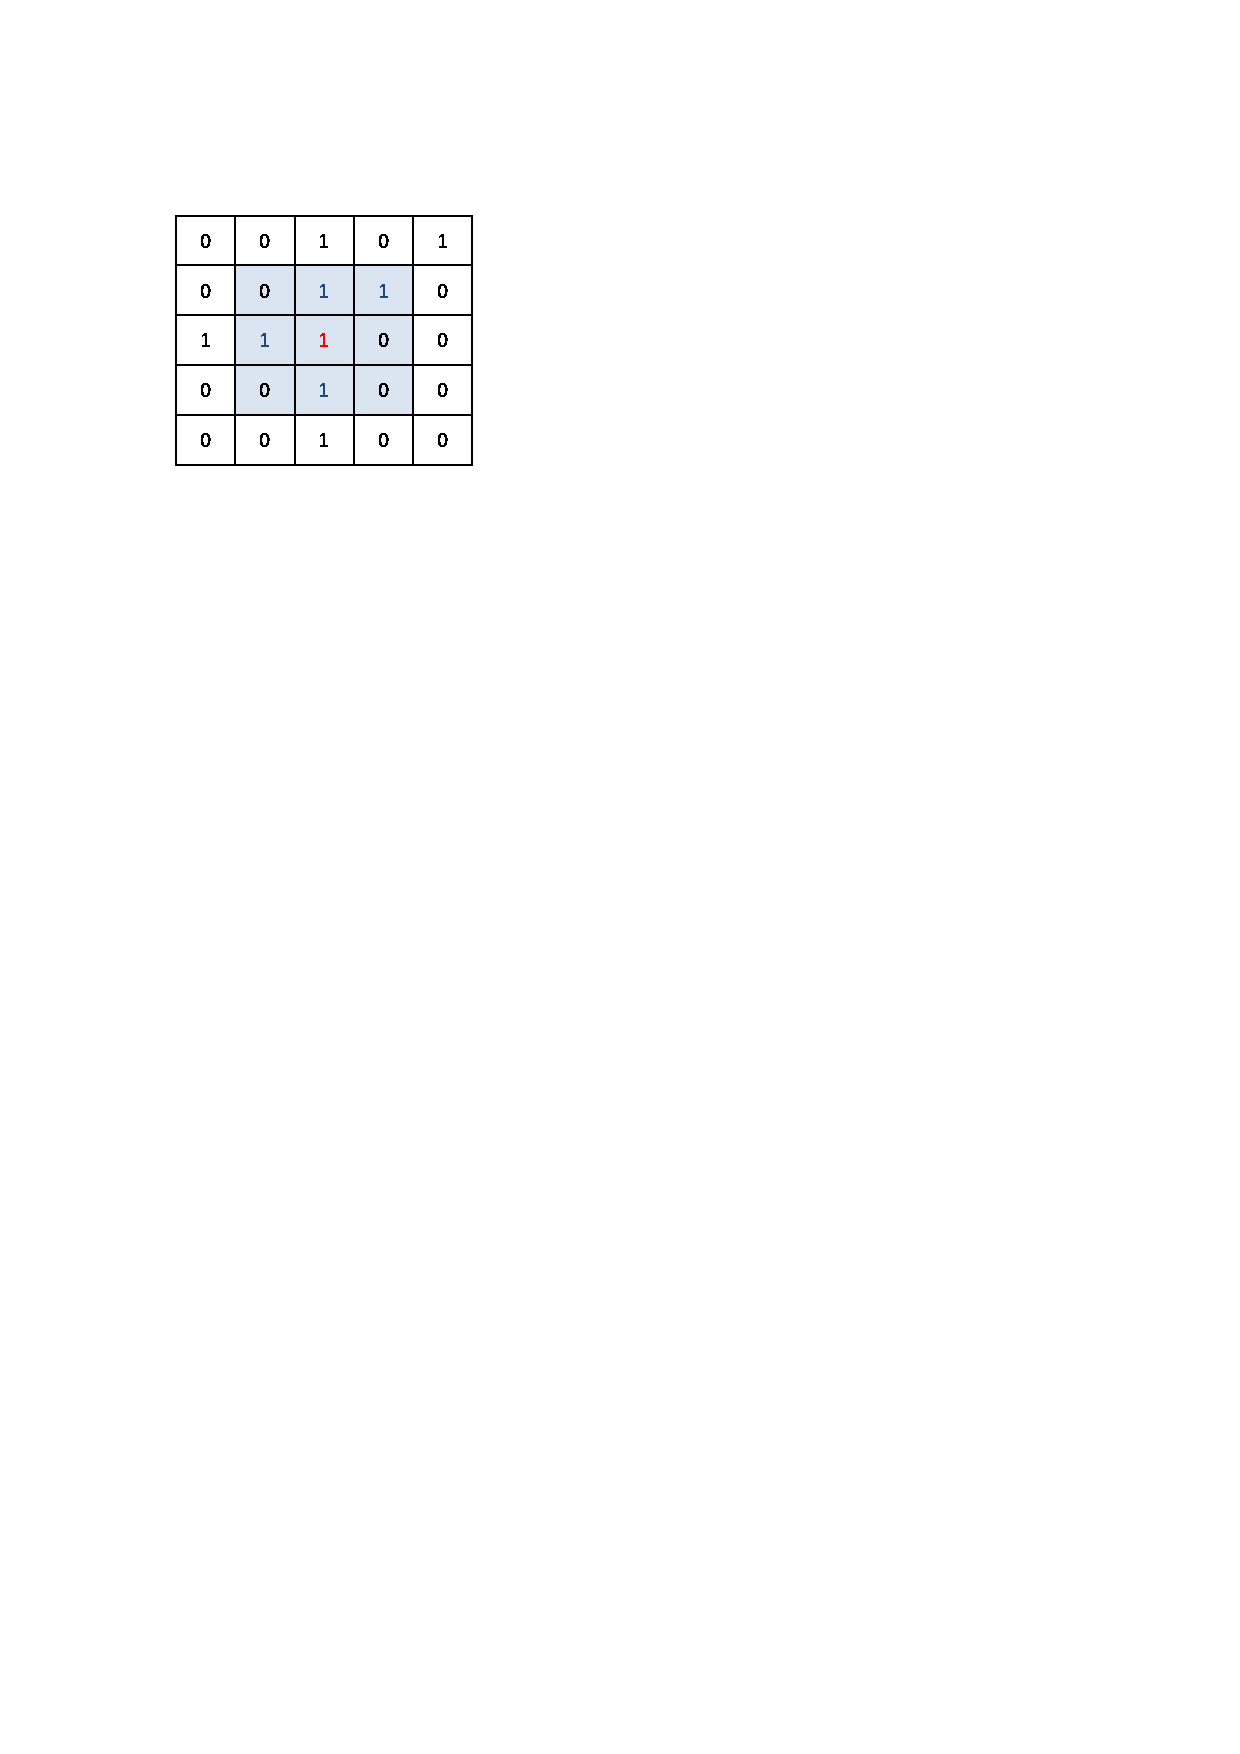
\includegraphics[width=4cm]{4FeaturePoint}
      \centerline{(b)}\medskip
	\label{fig:4FeaturePoint}
  \end{minipage}
\caption{三分叉点与四分叉点}
\label{fig:FeaturePoints}
\end{figure}

\begin{figure}
\centering
  \begin{minipage}[b]{1\textwidth} 
      \centering 
      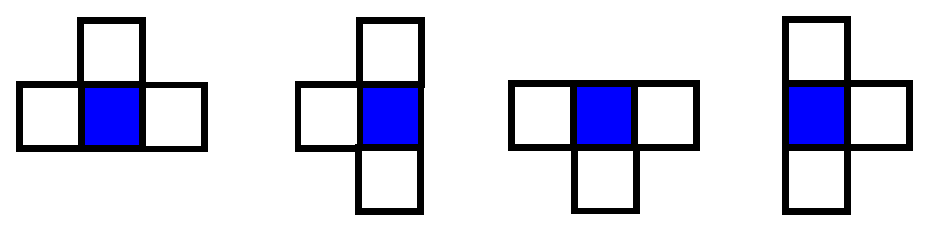
\includegraphics[width=8cm]{three-bifu}
        \centerline{(a)}\medskip
    \end{minipage}
  \begin{minipage}[b]{1\textwidth}
    \centering
    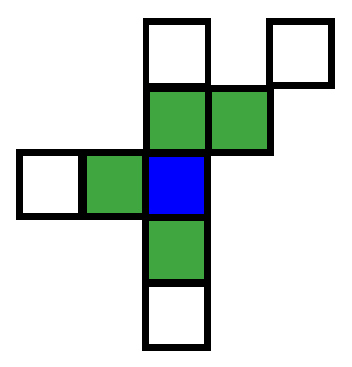
\includegraphics[width=3cm]{four-bifu}
      \centerline{(b)}\medskip
  \end{minipage}
\caption{三分叉点与四分叉点}
\label{fig:FeaturePoints-image}
\end{figure}

当所有的分叉点都检测到后,每个分叉点被看做一个种子,沿其八邻域像素值为1的方向不断向外扩展,直到找到与这个分叉点相邻的分叉点。遍历所有分叉点后,所有的分叉点及其连接关系就被检测到。为了方便后续操作,我们将采用顶点---边矩阵来表示分叉点及其连接关系,于是得到图\ref{fig:graph}的点---边关系表\ref{tab:AdjacentStructure},第一列为所有的分叉点,其余几列为与分叉点相连的分叉点。
\renewcommand\arraystretch{0.8}
\begin{table}
\caption{点——边关系}
\centering
\begin{tabular}{p{2cm}<{\centering}p{1cm}<{\centering}p{1cm}<{\centering}p{1cm}<{\centering}}
  \hline
  分叉点 & \multicolumn{3}{c}{相邻分叉点}\\
  \hline
  \rowcolor{gray!50}
  $v_{1}$ & $v_{2}$  & $0$      & $0$  \\
  $v_{2}$ & $v_{1}$  & $v_{3}$  & $v_{4}$ \\
  \rowcolor{gray!50}
  $v_{3}$ & $v_{2}$  & $v_{4}$  & $0$\\
  $v_{4}$ & $v_{2}$  & $v_{3}$  & $0$ \\
  \rowcolor{gray!50}
  $v_{5}$ & $0$      & $0$      & $0$\\
  \hline
\end{tabular}
\label{tab:AdjacentStructure}
\end{table}

众所周知,能够组成环结构的分叉点数目至少为3,这就要求每个分叉点的度大于等于3,即$d_{v_i} \geq 3$,并且每个分叉点应至少在点---边关系矩阵中出现3次。通过这个规则,可以滤除一些不能组成环结构的点。但这个过程不能一次滤除所有的不能组成环结构的无效点,而是需要进行循环滤除,每进行一次,最外围的无效点将会滤除,直到所有的无效点被滤除后,循环得以结束。以一个视网膜图像为例,如图\ref{fig:Bifurcation},分别表示初始检测到的分叉点与所有无效分叉点被滤除后的图像,从图中可以看出,分支末端的点都被滤除,只剩下可能组成环的分叉点。通过滤除不能组成环的无效的分叉点,就可以大大的减少搜索环的路径,从而减小环检索算法的复杂度。

\begin{figure}
\centering
  \begin{minipage}[b]{0.48\textwidth} 
      \centering 
      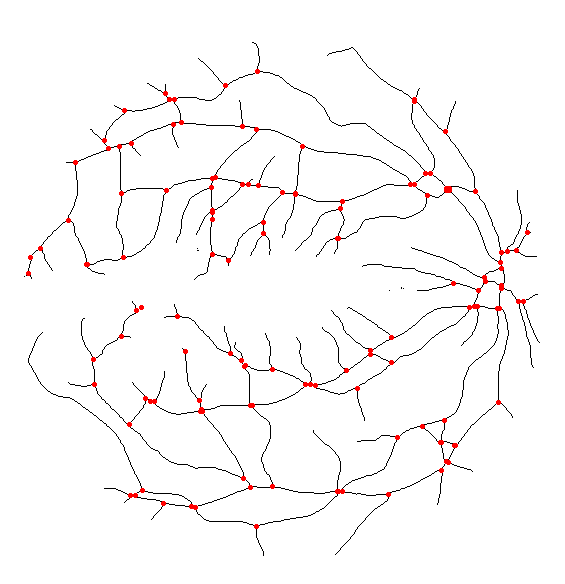
\includegraphics[width=4cm]{all-bifu}
        \centerline{(a)}\medskip
	 \label{fig:3FeaturePoint}
    \end{minipage}
  \begin{minipage}[b]{0.48\textwidth}
    \centering
    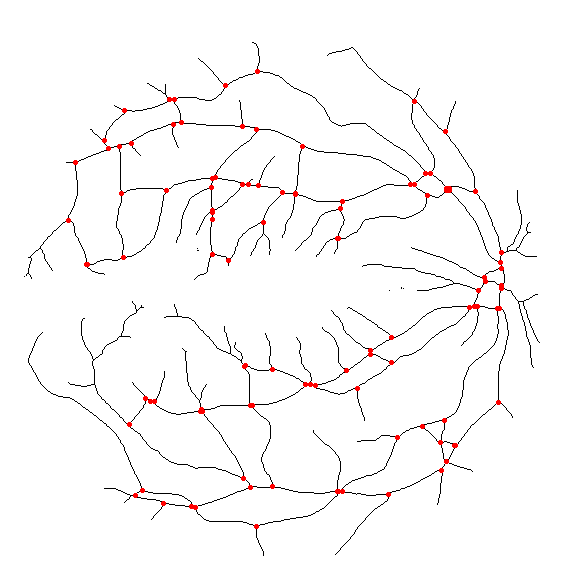
\includegraphics[width=4cm]{select-bifu}
      \centerline{(b)}\medskip
	\label{fig:4FeaturePoint}
  \end{minipage}
\caption{三分叉点与四分叉点}
\label{fig:Bifurcation}
\end{figure}

\subsubsection{检测环状结构}
\label{}


在图中检测最小环基的问题实际上是图论中的一个被广泛研究的问题。我们提出了动态路径移动算法,该算法的主要思想是把点--边邻接矩阵转化为一个树结构,然后通过树结构检测环结构。

树的定义如下:
树是包括n个结点的有限集合$T(n \geq 1)$\cite{zhangming},使得
\begin{enumerate}
\item 有且只有一个特定的成为根的结点。
\item 除根以外的其他结点被分成m个$(m \geq 0)$个不相交的有限集合$T_1, T_2, \ldots, T_m$,而没一个集合又都是树。其中,树$T_1, T_2, \ldots, T_m$称作这个根的子树。
\end{enumerate}

这个定义是递归的,即在树的定义中又用到了树的概念。在一棵树中,若存在节点k指点个结点$k'$的连线,则称k是$k'$的父结点,而$k'$是k的子结点,有向连线$<k, k'>$称作边。同一个父结点的子结点之间称为兄弟。树中没有父结点的结点称为根,没有子结点的结点称为树叶。若树中存在结点序列$k_0,k_1,\ldots,k_s$,使得$<k_0,k_1>,<k_1,k_2>,\ldots,<k_{s-1},k_s>$都是树中的边,则称从结点$k_0$到结点$k_s$存在一条路径。若有一条由k到达$k_s$的路径,责成k是$k_s$的祖先,$k_s$是k的子孙。图\ref{fig:tree}表示一棵树,A表示根结点,B、C是A的子结点,A是BC的父结点。ABDI是一条路径,其中A是I的祖先,I为A的子孙。

\begin{figure}[!ht]
\centering
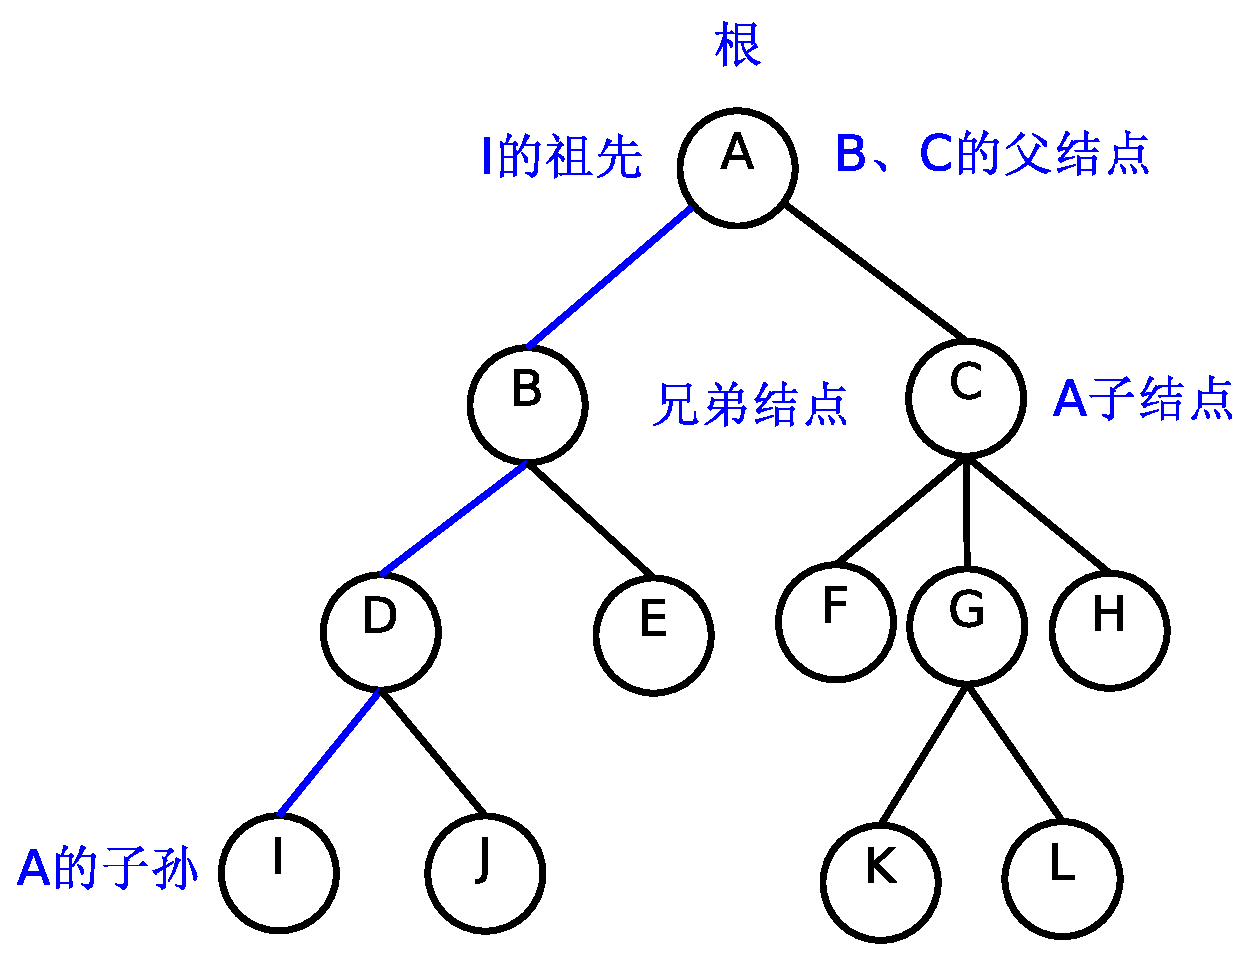
\includegraphics[width=0.3\textwidth]{tree-1}
\caption{树形表示法}
\label{fig:tree}
\end{figure}

动态路径移动算法的主要步骤为:
\begin{enumerate}
\item 初始化一个顶点作为树的根。
\item 找到与这个顶点相邻的其他顶点,并把他们作为根的子结点,放入树的第二层。相邻的点可以通过点边邻接矩阵得到,因为它列出了与某一点相邻的所有的顶点。
\item 继续找与第一后代中的顶点相邻的点,作为树的第三层。在搜索根的子结点的相邻点的过程中,以排除其上一层中的点,即根结点不作为树的第三层中的点。
\item 判断树的第三层中的点是否在树中存在两次。若是,则意味着一个环结构产生了,那么这个点与其父结点直到祖先将会作为能组成环的点被输出。然后这个点将会被认为是树叶,不再继续寻找它的相邻点作为下一后代。
\item 判断当前层是否有不是树叶的结点,若有,则继续寻找它的相邻点作为第四层。
\item 重复第四步及第五步直到当前层所有的点都是树叶。
\end{enumerate}
经过以上步骤,所有三点、四点、五点环将被检测到。如图\ref{fig:cycle-tree}(a)是一个图的例子,图中有一个三点环、一个四点环、一个五点环。通过动态路径移动算法,这三个环要被准确无误的检测出来。首先确定$v_1$为初始点,即树的根。通过点边关系可得,与之相邻的点分别为$v_2, v_5, v_6, v_8$,于是,这四个点将被当作根的子结点放入树的第二层。继续寻找这四个点的相邻点,放入树的第三层。检测第三层中的点在当前树,即前三层中的存在次数,发现$v_5, v_6, v_7$都存在两次,于是,这三个点分别与他们的父结点及其祖先组成环,即$v_{1}v_{5}v_{6}$组成三点环,$v_{1}v_{6}v_{7}v_{8}$组成四点环。那么这些点将被当作树叶不再继续寻找与之相邻的点。而第三层中的其他点将继续寻找与之相邻的点,这个例子中,$v_4, v_3$分别被检测到,作为树的第四层。然后继续判断第四层中的点在当前树,即前四层中的次数,发现都出现两次,于是这两个点与其父结点、祖先形成一个新的环,即$v_{1}v_{2}v_{3}v_{4}v_{5}$组成五点环,$v_4, v_3$将被作为树叶,不再继续往下寻找。至此,所有的搜索都已完成,即共找到三个环,$v_{1}v_{5}v_{6}$组成三点环,$v_{1}v_{6}v_{7}v_{8}$组成四点环,$v_{1}v_{2}v_{3}v_{4}v_{5}$组成五点环。

\begin{figure}
\centering

  \begin{minipage}[b]{1\textwidth} 
      \centering 
       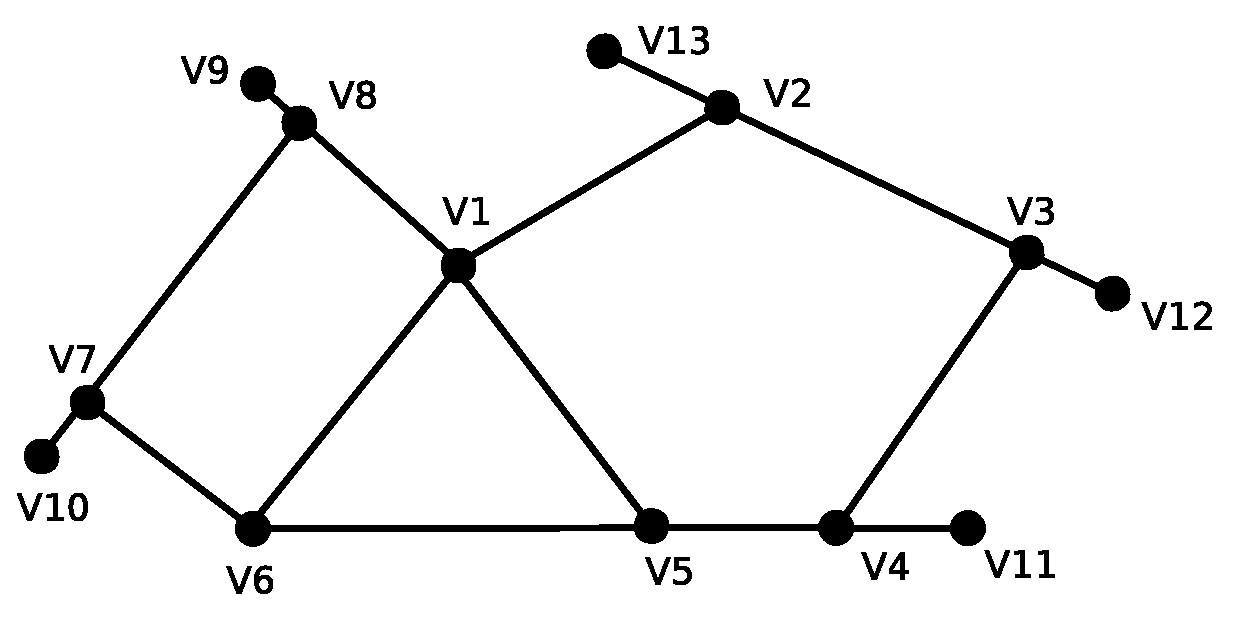
\includegraphics[width=7cm]{graph2}
       \centerline{(a)}\medskip
    \end{minipage}
  \begin{minipage}[b]{1\textwidth}
    \centering
    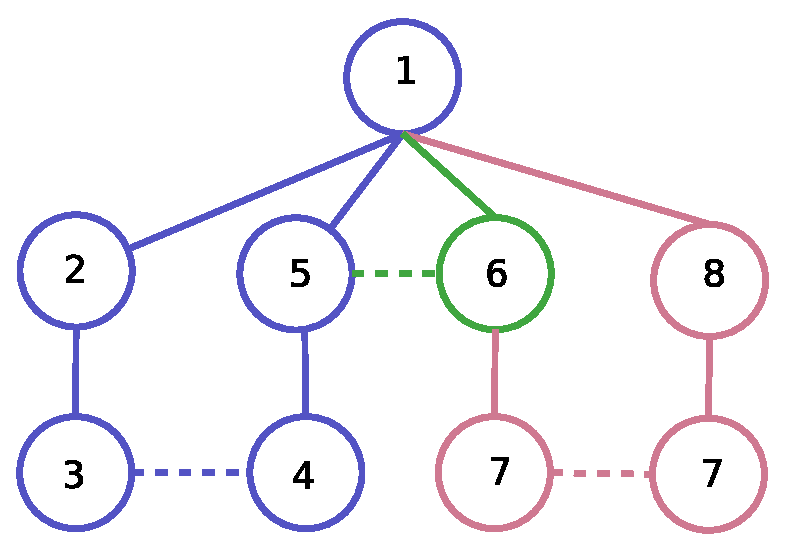
\includegraphics[width=6cm]{tree}
    \centerline{(b)}\medskip
  \end{minipage}
\caption{环结构与树结构}
\label{fig:cycle-tree}
\end{figure}

\subsubsection{特征描述}
\label{}
环之所以能用在图像识别与匹配领域,是因为它是稳定的显著的特性。而它的稳定性与显著性则体现在用来描述环结构的特征向量上。

一个环结构是由一系列分叉点与连接这些分叉点之间的线组成。我们用分支角度与分支长度来描述环结构。以任意分叉点$v_i(x_0, y_0)$为中心,构造一个$7 \times 7$的邻域。记录分支与邻域边缘24个像素相交点的坐标,假设其坐标值为$x_j, y_j, j=1, 2, \ldots$。则分支方向为:
\begin{align}
\beta_j = arctan\frac{dy}{dx}, dy = y_j - y_0, dx = x_j - x_0 
\end{align}

由于arctan的取值范围为$-90^{\circ} \sim 90^{\circ}$,故还需保证求出的角度大于0。即
\begin{align}
\alpha_j = \left\{ \begin{array}{ll}
\beta_j & \textrm{$dy \geq 0$, $dx \geq 0$} \\
\beta_j + 180^{\circ} & \textrm{$dy \geq 0$, $dx \leq 0$ 或 $dy \leq 0$, $dx \geq 0$}\\
\beta_j + 360^{\circ} & \textrm{$dy \leq 0, dx \leq 0$}
\end{array} \right.
\end{align}
邻域边缘24个像素把$360^{\circ}$分成了24个离散值,每个相邻的分支角度相差$15^{\circ}$。每个角度以水平线为基准,故分叉点之间的角度值可通过式\ref{eq:Angle}计算:
\begin{align}
\theta_i = \alpha_{i+1} - \alpha_i, \qquad
\theta_i = \left\{ \begin{array}{ll}
\theta_i + 360^{\circ} & \theta_i \le 0 \\
\theta_i & \theta_i \geq 0
\end{array} \right.
\label{eq:Angle}
\end{align}
如图\ref{fig:calculate-angles},以三分叉点为中心划定一个$7\times7$邻域,邻域的边缘24个像素把$360^{\circ}$分为24个方向的角度,分别为$15^{\circ}, 30^{\circ},45^{\circ}, \ldots, 360^{\circ}$,这个邻域的边缘24个像素中,像素值为1的像素以水平线为基准与中心像素形成分支角度,图\ref{fig:calculate-angles}中,共形成3个角度,即$45^{\circ}, 150^{\circ},270^{\circ}$,则分支之间的角度为$105^{\circ}, 120^{\circ}, 135^{\circ}$。

\begin{figure}[!ht]
\centering
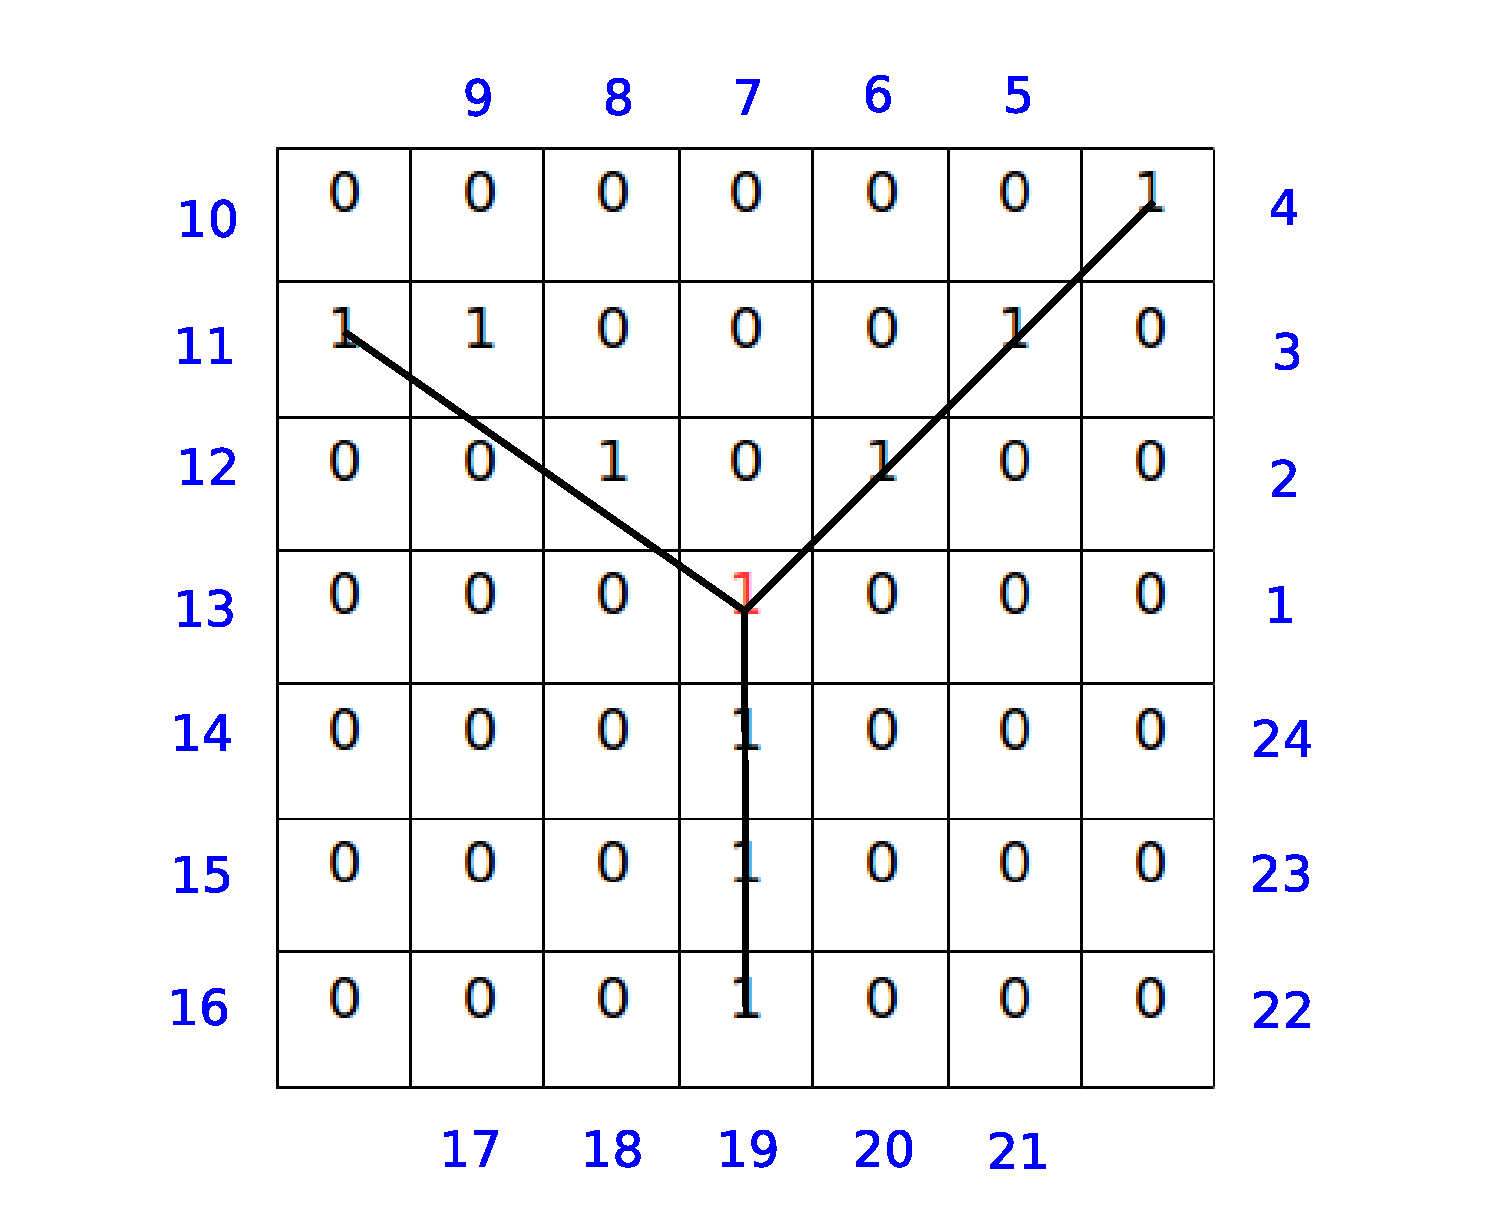
\includegraphics[width=0.5\textwidth]{figures/7-7}
\caption{分支角度计算}
\label{fig:calculate-angles}
\end{figure}

分叉点之间的分支长度为分叉点之间的欧式距离,即:
\begin{align}
L = \sqrt{(y_j - y_0)^2 + (x_j - x_0)^2}, j = 1, 2, \ldots
\end{align}

归一化属于数字信号处理范畴,即将有量纲的表达式,经过变换,转换为无量纲的表达式,成为标量。它是简化计算,缩小量值的有效办法。而对于环结构特征,通过归一化,能使在减少计算量的基础上,使环结构特征具有平移、旋转及尺度不变特征。图\ref{fig:description}给出了四点环结构示意图,角度归一化式\ref{eq:angle}、长度归一化式\ref{eq:length}及最终产生的特征向量可用式\ref{eq:vector}表示。$L_{1} \sim L_{4}$,$\theta_{1} \sim \theta_{14}$,$\theta_{15} \sim \theta_{18}$ 分别代表分支长度、分支角度及分叉点之间的角度。

\begin{figure}[!ht]
\centering
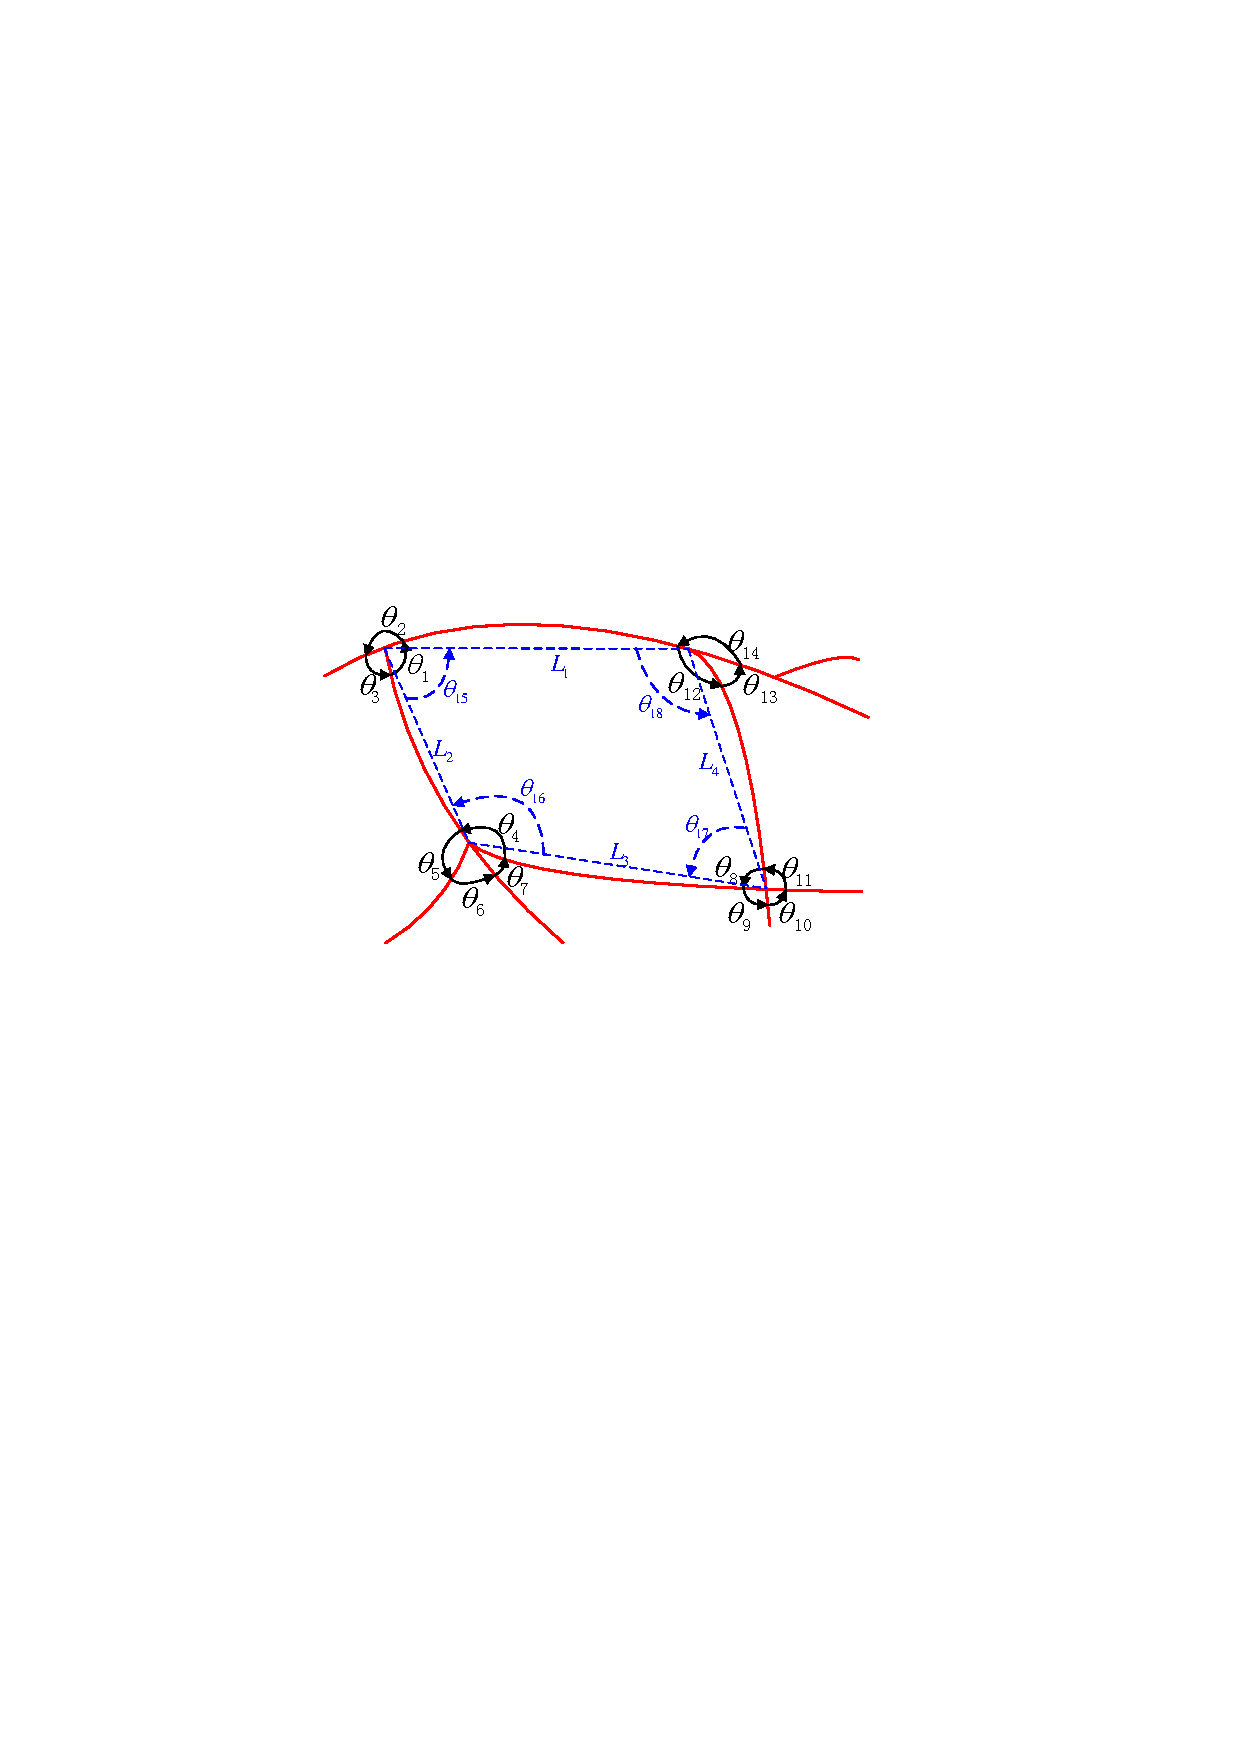
\includegraphics[width=0.4\textwidth]{figures/description.pdf}
\caption{环结构描述}
\label{fig:description}
\end{figure}
\begin{align}
L_{iNorm}&=\frac{L_i}{\sum{L}}\label{eq:length}\\
\theta_{jNorm}&=\frac{\theta_j}{360^\circ}\label{eq:angle}
\end{align}
\begin{multline}
\tilde{v}=\{\textrm{角度,长度}\}=\{L_{1},L_{2},L_{3},L_{4},\theta_{1},\theta_{2},\theta_{3},\mathbf{0},\theta_{4},\\\theta_{5},\theta_{6},\theta_{7},\theta_{8},\theta_{9},\theta_{10},\theta_{11},\theta_{12},\theta_{13},\theta_{14},\mathbf{0},\theta_{15},\theta_{16},\theta_{17},\theta_{18}\}
\label{eq:vector}
\end{multline}

值得注意的是,组成环的分叉点个数不一样,并且每个分叉点的分叉角度也不同,这就导致了不同类型的环有不同长度的特征向量。为了便于识别和配准的需要,我们可根据实际情况设定一个角度个数标准,比如说,若设置4个分支角度为标准,那么小于4个角度的分叉应用0来补齐,这样就保证同种类型的环的特征向量的长度是相同的。这样,当用来做配准或识别时,就可匹配同种类型的环的特征向量来达到目的。

\section{本章小节}
\label{}

本章介绍了环结构特征的定义、特点及应用,阐述了从图像中检测环的主要步骤:检测分叉点及其连接关系、滤除无效分叉点、检测环结构,并重点介绍了我们提出的动态路径移动算法。同时,结合环结构的特点,给出了特征描述的方法。通过把环结构特征表示成为特征向量,就能为下一步的配准、识别奠定基础。
